\documentclass[SE,lsstdraft,authoryear,toc]{lsstdoc}
\input{meta}

% Package imports go here.

% Local commands go here.

%If you want glossaries
%\input{aglossary.tex}
%\makeglossaries

\title{Surface brightness profiles around massive galaxies from LSSTCam coadds}

% This can write metadata into the PDF.
% Update keywords and author information as necessary.
\hypersetup{
    pdftitle={Surface brightness profiles around massive galaxies from LSSTCam coadds},
    pdfauthor={ConghaoZhou},
    pdfkeywords={}
}

% Optional subtitle
% \setDocSubtitle{A subtitle}

\input{authors}

\setDocRef{SOTN-007}
\setDocUpstreamLocation{\url{https://github.com/lsst-so/sotn-007}}

\date{\vcsDate}

% Optional: name of the document's curator
% \setDocCurator{The Curator of this Document}

\setDocAbstract{%
Low surface brightness photometry of massive galaxies can probe their extended stellar halos and the intracluster light but is often limited by background subtraction and masking systematics. Here we present radial surface brightness profiles for 15 massive brightest cluster galaxies selected from the Hyper Suprime-Cam (HSC) S16A massive-galaxy catalog. The profiles are measured in LSSTCam Data Preview 2 coadds produced with two different background treatments (\texttt{deep\_coadd} and \texttt{pretty\_coadd}). To make the comparison as direct as possible, the DP2 profiles are measured with the same per-galaxy source masks and on the same radial bins as the HSC photometry. The surveys are therefore compared bin by bin on a common pixel set. The HSC profiles are measured on images from the third HSC public data release, whose own two-stage sky subtraction we summarize. The \texttt{deep\_coadd} profiles match HSC to within $0.05$ mag arcsec$^{-2}$ inside $3''$ but become progressively fainter outward. The deficit is $0.15$ mag arcsec$^{-2}$ at $3''$--$5''$ and $0.5$ mag arcsec$^{-2}$ beyond $10''$, with a median of $0.21$ over $3''$--$40''$. This is the signature of background over-subtraction, which removes the galaxies' own outer light. The measured intensity falls to zero and the profiles end at a median semi-major axis of $18''$, against $63''$ for HSC. The \texttt{pretty\_coadd} profiles reach further out but behave inconsistently. For four of the eight galaxies where they extend beyond $20''$ they flatten into a plateau $1.4$--$2.1$ mag arcsec$^{-2}$ brighter than HSC. We show this plateau to be residual sky in the \texttt{pretty\_coadd} rather than recovered low surface brightness flux.}

% Change history defined here.
% Order: oldest first.
% Fields: VERSION, DATE, DESCRIPTION, OWNER NAME.
% See LPM-51 for version number policy.
\setDocChangeRecord{%
  \addtohist{1}{YYYY-MM-DD}{Unreleased.}{Zhou}
}

\begin{document}

% Create the title page.
\maketitle
% Frequently for a technote we do not want a title page  uncomment this to remove the title page and changelog.
% use \mkshorttitle to remove the extra pages

\section{Introduction}
The deep and wide photometric data provided by LSST open significant opportunities for low surface brightness (LSB) science, but the extent to which we can push our photometry depends sensitively on the accuracy of the background modeling. In particular, there can be background over- or under-subtraction near bright sources, and large-scale backgrounds that are scientifically interesting (e.g., the intracluster light) are often removed if not treated carefully. The massive central galaxies in galaxy clusters are a good test bed for these effects. They have large extended stellar envelopes that can be traced down to low surface brightness and they live in crowded fields. The photometry in their outskirts is therefore particularly sensitive to both the background modeling and the treatment of blended neighbors. In a previous note we measured surface brightness profiles for two massive galaxies in LSSTComCam Data Preview 1 and compared them to DECaLS precursor data \citedsp{SITCOMTN-165}. In this note we extend that analysis to LSSTCam Data Preview 2 (DP2). We measure surface brightness profiles for 15 massive brightest cluster galaxies (BCGs) in two DP2 coadd flavors produced with different background treatments. We compare them against profiles previously measured on Hyper Suprime-Cam (HSC) imaging of the same galaxies. We measure the DP2 profiles with the same per-galaxy source masks and on the same radial bins as the HSC photometry so that the comparison isolates the imaging and the background treatment rather than the analysis choices.

\section{Data} \label{sec:data}
The Rubin data we use in this note are LSSTCam DP2 coadds from the \texttt{LSSTCam/runs/DRP/DP2} collection. They are on the \texttt{lsst\_cells\_v2} sky map, a rings sky map with a pixel scale of $0.2''$ per pixel. Its tracts are $30000 \times 30000$ pixels ($1.67^\circ$ on a side) and overlap their neighbors by $1'$. Each tract is divided into $10 \times 10$ patches of $3000 \times 3000$ inner pixels ($10'$ on a side) with a $150$-pixel border. We use two coadd data products, \texttt{deep\_coadd} and \texttt{pretty\_coadd}, produced by the LSST Science Pipelines at versions v30.0.8 and v30.0.7 respectively. Both are assembled from the same selected visits, those with a PSF FWHM below $1.8''$, with the same Lanczos-3 warping. Both use the same coaddition, a $3\sigma$-clipped mean over two iterations with the compare-warp artifact rejection. In both, the pixels flagged as bad, saturated, or without data are interpolated over. Neither carries a bright-object mask or any bright-star subtraction, so the difference between them is entirely in the background treatment. 

The \texttt{deep\_coadd} is the standard Data Release Processing coadd on which detection and measurement are run. Its input visit images carry the per-detector sky subtraction of single-frame processing, an Akima-spline background on $128$-pixel ($25.6''$) bins. After coaddition a further background of the same form, again on $128$-pixel bins, is fitted and removed from the coadd before detection. In the pipeline's own description this coadd-level background intentionally over-subtracts in order to reduce blending between footprints and to ensure that scattered light is removed. Its $25.6''$ scale is close to the $21.5''$ scale of the HSC local sky subtraction described below. The HSC profiles in this note deliberately avoid that step by using the globally subtracted coadds. The \texttt{deep\_coadd} therefore corresponds to the HSC detection coadd, not to the product on which the HSC profiles in this work are measured. The deep-versus-HSC comparison below is thus a comparison of a locally subtracted image against one without that step. 

The \texttt{pretty\_coadd} is built from the same visits but with the per-detector background replaced by the full-focal-plane sky correction of the pipeline. This first subtracts a scaled sky frame. A sky frame is a template of the static response of the instrument to blank sky in that filter, built by stacking many dithered science exposures with sources masked. It captures the fixed patterns of the illumination and filter response rather than any real object. The template is scaled to the sky level of each exposure and subtracted. It then fits and removes two smooth focal-plane models on scales of about $27'$ and $14'$. This treatment preserves structure on the scale of a detector and below at the cost of being more affected by scattered light and other instrumental backgrounds. No coadd-level background is removed from it. Its purpose in the pipeline is the production of color images. The two products therefore bracket the background treatment. The \texttt{deep\_coadd} is the more aggressively flattened image. The \texttt{pretty\_coadd} keeps extended light together with whatever residual sky and scattered light survives the larger-scale model. Comparing them on the same pixels through the same masks probes how much the background subtraction affects the galaxy outskirts. For each galaxy we extract a $160'' \times 160''$ cutout centered on the catalog position in the highest-priority band ($r$, then $i$, then $g$) that is available and usable in both coadd types at that position.

The comparison data come from the third public data release of the HSC Subaru Strategic Program \citep[PDR3;][]{2022PASJ...74..247A}, whose Wide layer reaches $\sim 26$\,mag at $5\sigma$ over $670$\,deg$^2$ at full depth in $grizy$. PDR3 is processed with \texttt{hscPipe}~8, which subtracts the sky in two stages. A global sky subtraction is applied before coaddition in three steps. First, an $8\mathrm{k} \times 8\mathrm{k}$-pixel ($\sim 23'$) background is removed from each visit to take out exposure-specific large-scale gradients such as scattered light. Second, a scaled sky frame of the kind described above is subtracted. It is normalized from typically more than 50 visits with large dithers, and in PDR3 it includes large-scale static features as well as the structure within a superpixel. Third, a further subtraction is made on $256$-pixel superpixels. These globally subtracted coadds are designed to keep the wings of bright sources and are the products intended for the study of extended objects. A second and deliberately more aggressive local sky subtraction is then applied immediately before the detection and measurement stages on $128$-pixel superpixels ($\sim 21.5''$). It intentionally removes the wings of bright objects in order to limit footprint blending and deblending failures. This is the change relative to PDR1 and PDR2 that significantly reduced the number of false detections. The two stages produce different coadd images.

Our targets are drawn from the HSC S16A massive-galaxy catalog with $\log M_\star/M_\odot > 11.2$ \citep{huangOuterStellarMass2022}. That catalog carries a cross-match to the redMaPPer cluster catalog described by \citet{huangOuterStellarMass2022}. This is an internal redMaPPer run on the HSC S16A data. It uses the updated Python implementation of the algorithm with the same approach as the DES run of \citet{2016ApJS..224....1R} apart from minor modifications. Over $0.19 < z < 0.52$ it contains 2409 clusters with richness $\lambda \ge 5$ (227 with $\lambda \ge 20$). Two thirds of them have spectroscopic redshifts and the remainder have red-sequence photometric redshifts with a scatter of $\sigma_z/(1+z) \simeq 0.011$ for $\lambda \ge 5$. For each cluster the central galaxy is the candidate with the highest redMaPPer centering probability $P_\mathrm{cen}$. In this HSC sample 66\% of clusters have a central with $P_\mathrm{cen} > 0.8$. For each massive galaxy the catalog records the matched cluster, its richness, and whether the galaxy is that cluster's central. We select the galaxies flagged as cluster centrals with clean photometry and cross-match them against the tracts processed in DP2. The overlap is the equatorial strip at $\mathrm{RA} \simeq 330$--$341^\circ$, $\mathrm{Dec} \simeq -1$ to $+2^\circ$. We keep the 15 matched BCGs with redMaPPer richness $\lambda \ge 5$, spanning $z = 0.24$--$0.51$. The richest matched system has $\lambda = 9$, so the sample probes groups and poor clusters rather than massive clusters.

The comparison profiles are surface brightness profiles measured with \texttt{isoster}, an accelerated elliptical isophote fitter, directly on the HSC $g$, $r$, and $i$ coadd images of the same galaxies in a separate analysis (Wei et al., in preparation). These are calibrated $\mu(r)$ profiles in AB mag\,arcsec$^{-2}$ with uncertainties on a fixed logarithmic grid of semi-major axis (SMA) values. The DP2 comparison is made in the same band as the HSC profile wherever possible. That analysis also provides the per-galaxy source mask used for the photometry of each galaxy, which we reuse here. The HSC profiles are measured on the coadds before the local stage. These are the globally sky-subtracted patch coadds that PDR3 stores under \texttt{deepCoadd/}, the \texttt{coadd/bg} product of the HSC cutout service. The locally subtracted \texttt{calexp} coadds used for detection are avoided because they show a slight over-subtraction near bright sources caused by the local stage. Mock tests indicate that the globally subtracted coadds are in turn slightly under-subtracted. The HSC measurement pipeline (\texttt{MassiveCat}) therefore applies one additional local sky estimate before fitting. It is a two-dimensional tilted plane, $I(X,Y) = I_0 + X\,\delta_x + Y\,\delta_y$, fitted with \textsc{AstroPhot} \citep{2023MNRAS.525.6377S}, where $I_0$ is the central sky level and $\delta_x$, $\delta_y$ are its gradients. The HSC background is therefore a large-scale global model plus a first-order local plane with no subtraction on the $\sim 21.5''$ scale of the local stage. That is the relevant point of contrast with the DP2 coadds in the comparison below.

\section{Surface brightness profile}
In this section we describe the method we use to extract surface brightness profiles from the DP2 coadds. We mask every source other than the BCG with exactly the per-galaxy source mask used for the HSC \texttt{isoster} photometry so that the two surveys are measured through the same mask. These are the \texttt{mask\_fit} images on the HSC $0.168''$ pixel grid, built by \texttt{MassiveCat} from the HSC-I image as follows. A base mask combines the HSC pipeline's \texttt{DETECTED}, \texttt{BAD}, \texttt{SAT}, and \texttt{NO\_DATA} pixels. Because the PDR3 bright-star mask is too aggressive, a bright-star mask is built independently from Gaia DR3. Each selected star is masked with a circle whose radius follows Equation~2 of \citet{2018PASJ...70S...7C}, $r(G) = 708.9\,\exp(-G/8.41)$ arcsec for $G < 9$ and $694.7\,\exp(-G/4.04)$ arcsec for $G \ge 9$. The union of the two is the starting point for a source-detection pass. The image is smoothed with a Gaussian kernel of FWHM 3 pixels. Connected regions of at least 8 pixels above the $1\sigma$ global noise level are then detected and dilated by 5 pixels. The result is the mask used for sky estimation, the \texttt{mask\_sky} product. The fitting mask starts from that sky mask, removes the central target from it, and keeps the bright-star and bad-pixel regions. It then adds the sources blended into the target, which are found on unsharp-masked residual images. Each residual is the image minus a Gaussian-smoothed copy of itself, and two smoothing scales are used, FWHM 15 and 70 pixels. On each residual image connected regions of at least 8 pixels above $5\sigma$ are detected and deblended, and each detection is expanded by 2 pixels. The detections from the two scales are combined and the result is dilated by 5 pixels. The result retains the target galaxy while masking the neighbors blended into it and is what \texttt{mask\_fit} contains. For each galaxy the HSC mask is reprojected onto the DP2 stamp by a nearest-neighbor lookup through the two WCSs. Every DP2 pixel is mapped to the sky with the DP2 WCS and to the nearest HSC mask pixel with the HSC WCS. The HSC cutouts ($\sim 200''$ across) are larger than the $160''$ DP2 stamps, so the reprojected mask covers the whole stamp. Because the HSC masks know nothing about LSSTCam defects, the reprojected mask is combined with the DP2 non-detection mask planes (\texttt{NO\_DATA}, saturation, etc.) of both the \texttt{deep\_coadd} and the \texttt{pretty\_coadd} stamps. The two coadd types are then fitted on one identical pixel set. The masks cover 23--48 percent of each stamp (median 34 percent) or 23--64 percent (median 38 percent) once the DP2 bad planes are added. The band is chosen with the $r$, $i$, $g$ priority described above, skipping a band if the combined mask covers the BCG center or more than 98 percent of the stamp.

We measure the profiles with \texttt{isoster}. For each galaxy and coadd type we first run a free-growing fit, with center, ellipticity, and position angle free per isophote, to establish the isophote geometry as a function of radius. We then re-extract the photometry in forced mode at exactly the SMA values of the HSC profile, using geometry interpolated from the free fit and clamped to the outermost fitted values beyond its reach. The DP2 and HSC profiles therefore share identical radial bins. The only bins missing on the DP2 side are those extending beyond the cutout for BCGs near a patch boundary. The fits use the coadd variance plane through weighted least squares, and the per-isophote uncertainty on the mean intensity is propagated into the surface brightness uncertainty. As in \citedsp{SITCOMTN-165}, we only show points with an intensity signal-to-noise ratio greater than 1. The same cut is applied to the HSC points, where it corresponds to an uncertainty $\sigma_\mu < 2.5/\ln 10 = 1.09$\,mag\,arcsec$^{-2}$. Both surveys are thus shown and compared at the same significance. The cut is applied after the radii are chosen, so the DP2 profiles are still measured at every radius the HSC profile defines rather than being truncated where HSC becomes noisy. All 15 BCGs are fitted successfully on \texttt{deep\_coadd} and 14 of 15 on \texttt{pretty\_coadd}. The exception is the $\lambda = 9$ system (42634963526383742), which is fitted in $g$ only and on \texttt{deep\_coadd} only because its \texttt{pretty\_coadd} $g$ stamp is entirely masked and there is no $r$ or $i$ coverage. In Figure~\ref{fig:examples} we show the masked cutouts and the resulting profiles for two representative galaxies, both compared in the $r$ band. In one of them the \texttt{pretty\_coadd} and HSC profiles agree over their common range. The other shows the \texttt{pretty\_coadd} plateau discussed below. In both galaxies the \texttt{deep\_coadd} profile falls below the HSC profile in the outskirts and ends early. This shows that the background subtraction of the \texttt{deep\_coadd} is too aggressive for extended galaxies.

\begin{figure}[htbp]
  \centering
  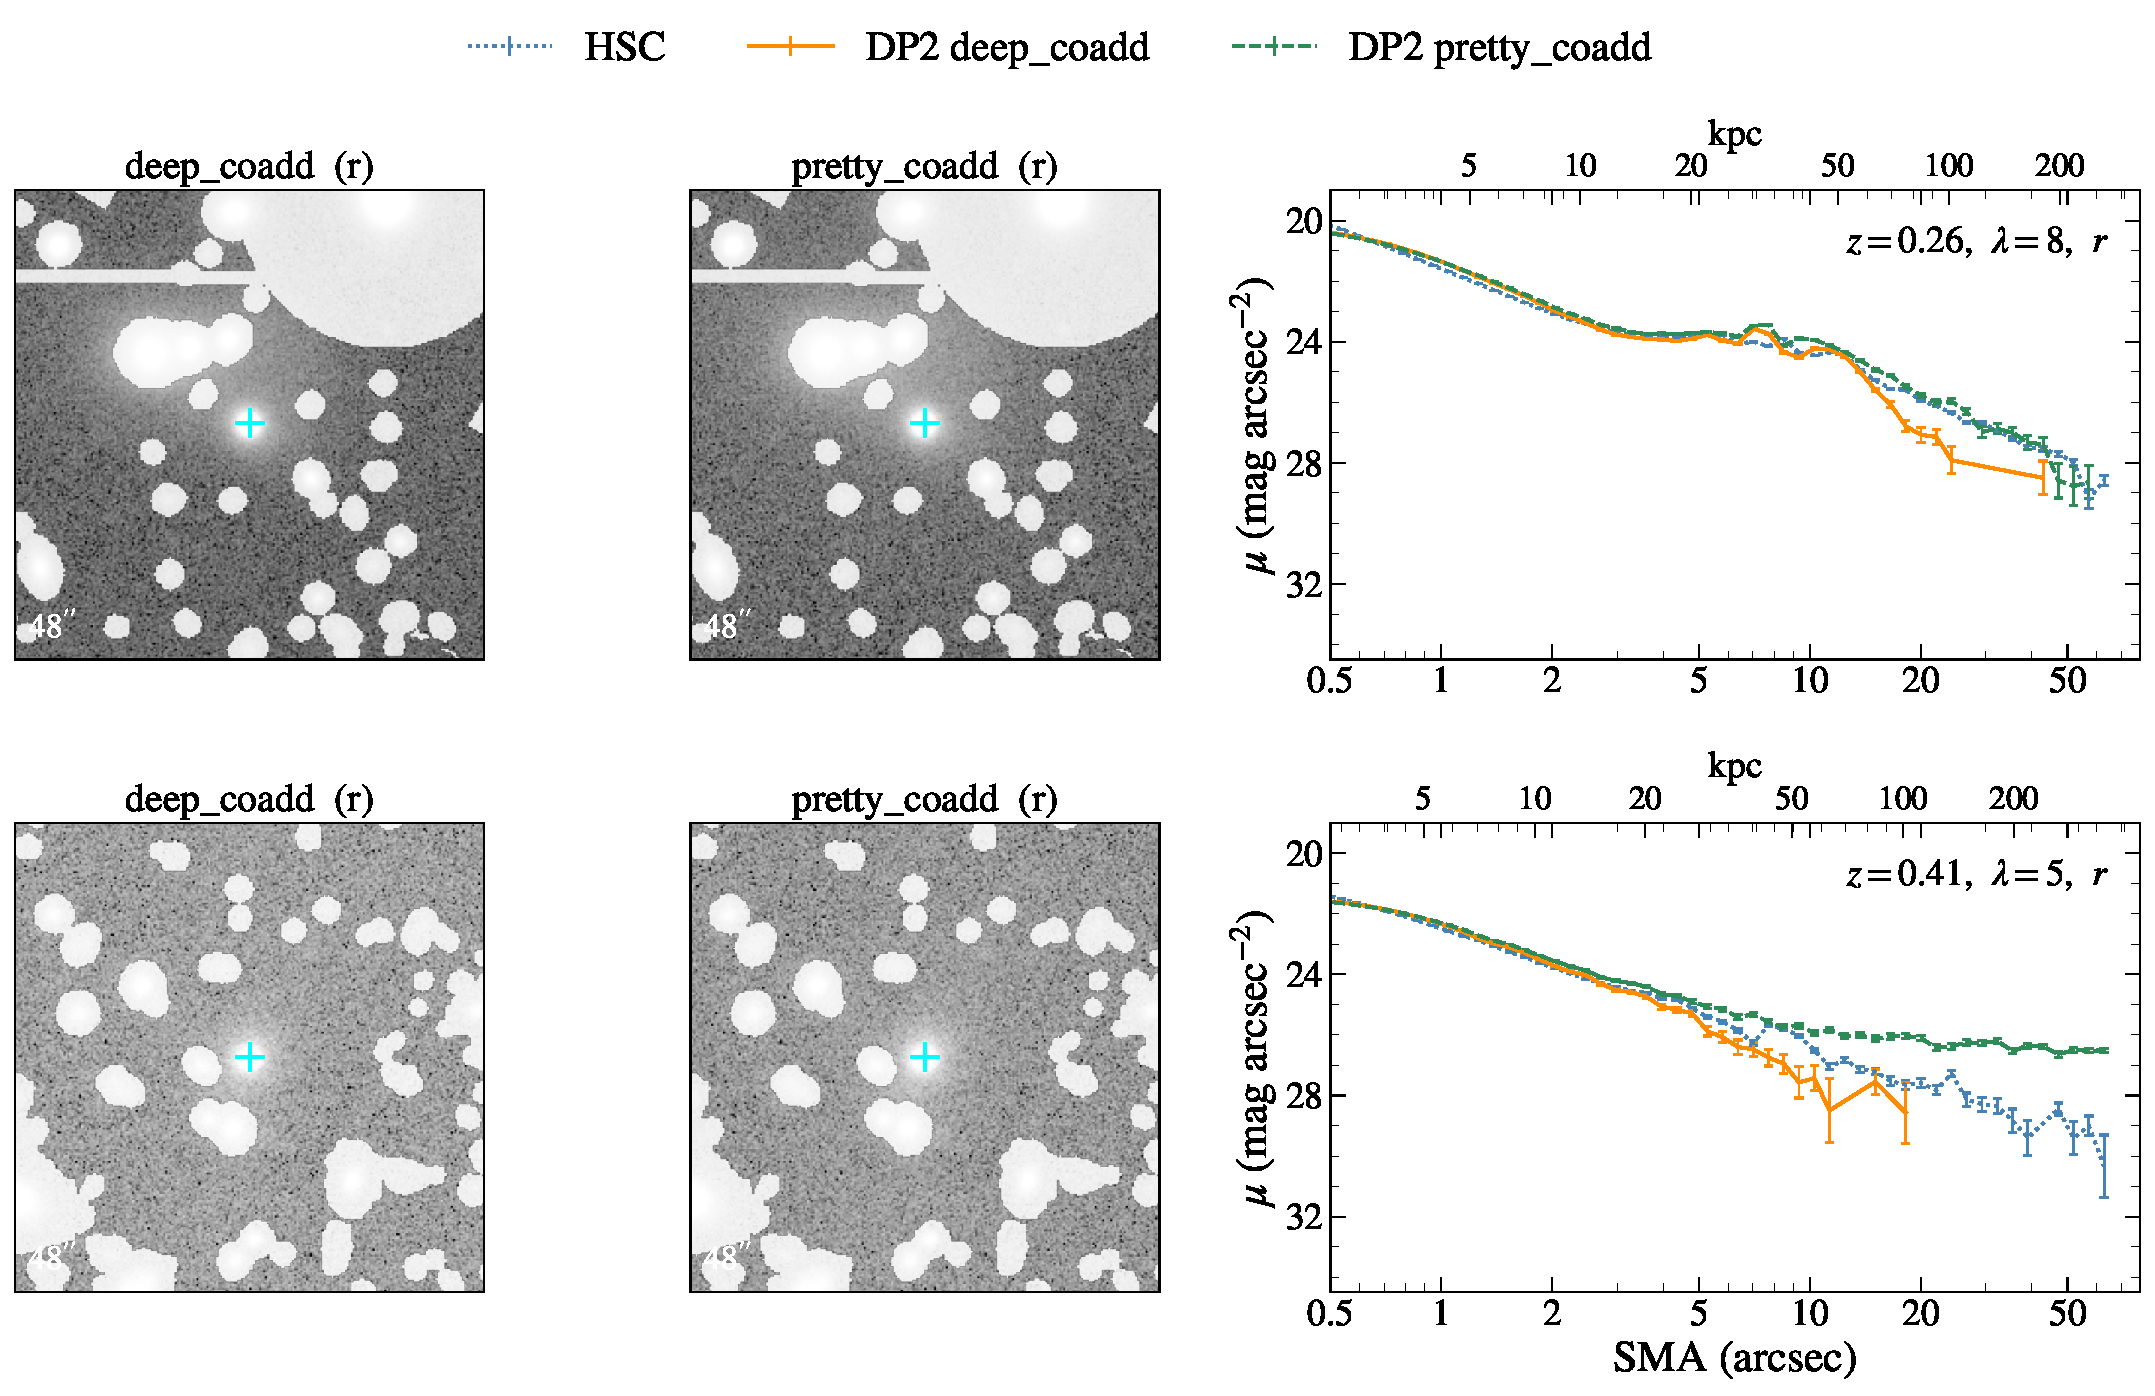
\includegraphics[width=1.0\linewidth]{figures/sbp_examples.pdf}
  \caption{Two representative BCGs. The top row shows a galaxy where the \texttt{pretty\_coadd} and HSC profiles agree over the whole range they have in common. The bottom row shows a galaxy with the \texttt{pretty\_coadd} plateau. Beyond $\sim 20''$ its profile flattens near $\mu \simeq 26.5$ mag\,arcsec$^{-2}$ and stays there to the edge of the stamp, while the HSC profile continues to decline over the same range, reaching $\mu \simeq 28$--$30$ mag\,arcsec$^{-2}$. The left and center panels show the \texttt{deep\_coadd} and \texttt{pretty\_coadd} cutouts, $48''$ across, through the reprojected HSC source mask. White regions are masked and the cyan cross marks the BCG. Both coadd types are fitted on the same pixel set. The right panels show the surface brightness profiles with $1\sigma$ uncertainties on identical radial bins for HSC (dotted blue), DP2 \texttt{deep\_coadd} (solid orange), and DP2 \texttt{pretty\_coadd} (dashed green). In both galaxies the \texttt{deep\_coadd} profile falls below HSC and ends earlier because its background subtraction is too aggressive. The over-subtraction drives the outer intensity to zero, below a signal-to-noise ratio of unity.}
  \label{fig:examples}
\end{figure}

\section{Comparison with HSC}
Figure~\ref{fig:all} shows the profiles for the whole sample and Figure~\ref{fig:examples} shows two representative cases in more detail. We quantify the agreement of two profiles by the median of $\Delta\mu = \mu_{\mathrm{DP2}} - \mu_{\mathrm{HSC}}$ over their common SMA bins between $3''$ and $40''$ so that positive values mean that the DP2 profile is fainter.

Inside $3''$, where the signal is strong, the DP2 and HSC profiles agree to within $0.05$\,mag\,arcsec$^{-2}$ for essentially all galaxies in all three bands. This rules out a calibration offset between the surveys. Beyond that the \texttt{deep\_coadd} profiles become progressively fainter than HSC. The median deficit is $0.15$\,mag\,arcsec$^{-2}$ at $3''$--$5''$, $0.32$ at $5''$--$10''$, and $0.5$ at $10''$--$40''$. Over $3''$--$40''$ the median is $0.21$\,mag\,arcsec$^{-2}$, with a 16th to 84th percentile range of $+0.12$ to $+0.45$ and a full range of $+0.03$ to $+0.61$\,mag\,arcsec$^{-2}$. An offset that is absent at the center and grows outward as the surface brightness falls is the signature of background over-subtraction. The $25.6''$ background model absorbs part of the galaxy's own extended light. The same effect sets where the profiles end. The over-subtracted intensity reaches zero and the profiles drop below a signal-to-noise ratio of unity at a median SMA of $18''$, against $29''$ for \texttt{pretty\_coadd} and $63''$ for HSC. The DP2 coadds here are $1.3$ to $1.8$\,mag shallower than HSC, so noise alone would also end the DP2 profiles early. The over-subtraction is nevertheless real. The $0.5$\,mag\,arcsec$^{-2}$ deficit at $10''$--$40''$ is a systematic offset in bins that pass the cut, and the \texttt{pretty\_coadd}, with the same visits and the same noise, reaches $29''$ against $18''$.

The \texttt{pretty\_coadd} profiles behave inconsistently and in their present form we do not consider them a reliable measurement of the outskirts. Their median offset from HSC is smaller, $+0.07$\,mag\,arcsec$^{-2}$, but the scatter is several times larger than for \texttt{deep\_coadd}. The 16th to 84th percentile range is $-0.57$ to $+0.31$ and the full range is $-0.91$ to $+0.50$\,mag\,arcsec$^{-2}$. The sign of the discrepancy varies from galaxy to galaxy. Eight galaxies have \texttt{pretty\_coadd} profiles that extend beyond $20''$. For four of them the profiles are $1.4$ to $2.1$\,mag\,arcsec$^{-2}$ brighter than HSC at those radii. More tellingly, they stop declining. Their logarithmic slopes over $r > 20''$ are $0.4$ to $1.2$\,mag\,dex$^{-1}$, against $1.0$ to $4.7$\,mag\,dex$^{-1}$ (median $4.0$) for the HSC profiles of the same galaxies. A profile that plateaus instead of declining is the signature of a residual background floor rather than of recovered galaxy light. The plateau level, $\mu \simeq 26$ to $28$\,mag\,arcsec$^{-2}$, is far brighter than where HSC still measures a declining profile for the same objects. Only two galaxies out of the eight agree with HSC at these radii (within $0.2$\,mag\,arcsec$^{-2}$), and those two do decline steeply with slopes of $5.9$ and $6.8$\,mag\,dex$^{-1}$. Of the remaining two, one is brighter than HSC by $1.0$\,mag\,arcsec$^{-2}$ but has only two bins beyond $20''$. The other is fainter than HSC by $1.0$\,mag\,arcsec$^{-2}$ over its outer bins and ends at $27''$. As we show next, both are effects of the residual sky of the \texttt{pretty\_coadd}. It is positive under the plateau galaxies, where it adds a floor, and negative under the last one, where it removes half or more of the galaxy's remaining light. We therefore caution that the brighter \texttt{pretty\_coadd} outskirts should not be read as LSB flux preserved by the gentler background treatment.

The plateau is in fact the residual sky of the \texttt{pretty\_coadd}. In the unmasked pixels $60''$--$80''$ from each BCG, the \texttt{deep\_coadd} stamps sit within $0.5$\,nJy per pixel of zero, whereas the \texttt{pretty\_coadd} stamps have residual levels between $-4.9$ and $+2.8$\,nJy per pixel. Since $1$\,nJy per pixel corresponds to $\mu = 27.9$\,mag\,arcsec$^{-2}$ at $0.2''$ per pixel, these residuals are at the brightness of the plateaus. For the four plateau galaxies the local residual is positive. Its surface brightness ($26.8$, $27.1$, $28.0$, and $28.1$\,mag\,arcsec$^{-2}$) matches the plateau level to within $0.4$\,mag\,arcsec$^{-2}$ since the plateau is the residual plus a little galaxy light. Where the residual is negative the outer profile is instead pushed fainter than HSC or below the signal-to-noise cut. This is the origin of both the large negative and the large positive \texttt{pretty\_coadd} offsets. Mapping the residual across whole patches in $100''$ cells shows that it is not a constant offset but a smooth ramp of up to $10$\,nJy per pixel across a $10'$ patch. This is structure on scales between the $25.6''$ background removed from the \texttt{deep\_coadd} and the $\sim 14'$ scale of the focal-plane sky correction. The \texttt{pretty\_coadd} inherits it from every visit. The \texttt{deep\_coadd} is flat to $0.05$\,nJy per pixel over the same patches. The \texttt{pretty\_coadd} profiles in this note should therefore be read as galaxy light plus residual sky.

Three further caveats apply to the comparison itself. First, the HSC profiles are not a background-neutral reference. As described in Section~\ref{sec:data}, they are measured on the globally sky-subtracted PDR3 coadds with an additional tilted-plane sky model removed. Every offset quoted here is therefore a difference between two background treatments rather than a measurement against ground truth. A tilted plane fitted over a $\sim 200''$ cutout is a first-order model, and any sky structure on scales between that plane and the global model remains in the HSC profile. By contrast, the \texttt{deep\_coadd} has had a $25.6''$-scale background removed and the \texttt{pretty\_coadd} retains residual sky on arcminute scales. Those differences are precisely what the outer offsets probe. Second, the limited radial extent of the DP2 profiles is set by the background treatment rather than by the masks, which are the same ones used for the HSC profiles. In the \texttt{deep\_coadd} the $25.6''$ coadd-level background removes the galaxy's own light beyond $\sim 15$--$20''$, so the isophote intensity there falls below the signal-to-noise cut and the profile ends. In the \texttt{pretty\_coadd} the residual sky of a few nJy per pixel varies in sign from field to field. It either lifts the outer profile into a plateau or, where negative, suppresses it below the cut. Third, five of the stamps cross a patch boundary and are clipped there, which removes the outermost HSC bins from the DP2 grid for those galaxies. We tested mosaicking the neighboring patches of the tract, which share its pixel grid, into full-size stamps. None of the \texttt{deep\_coadd} profiles change since all of them end well inside the clipped edge. Only three \texttt{pretty\_coadd} profiles extend further out into the residual-sky regime just described. We therefore keep the single-patch stamps in this note.

\begin{figure}[!htbp]
  \centering
  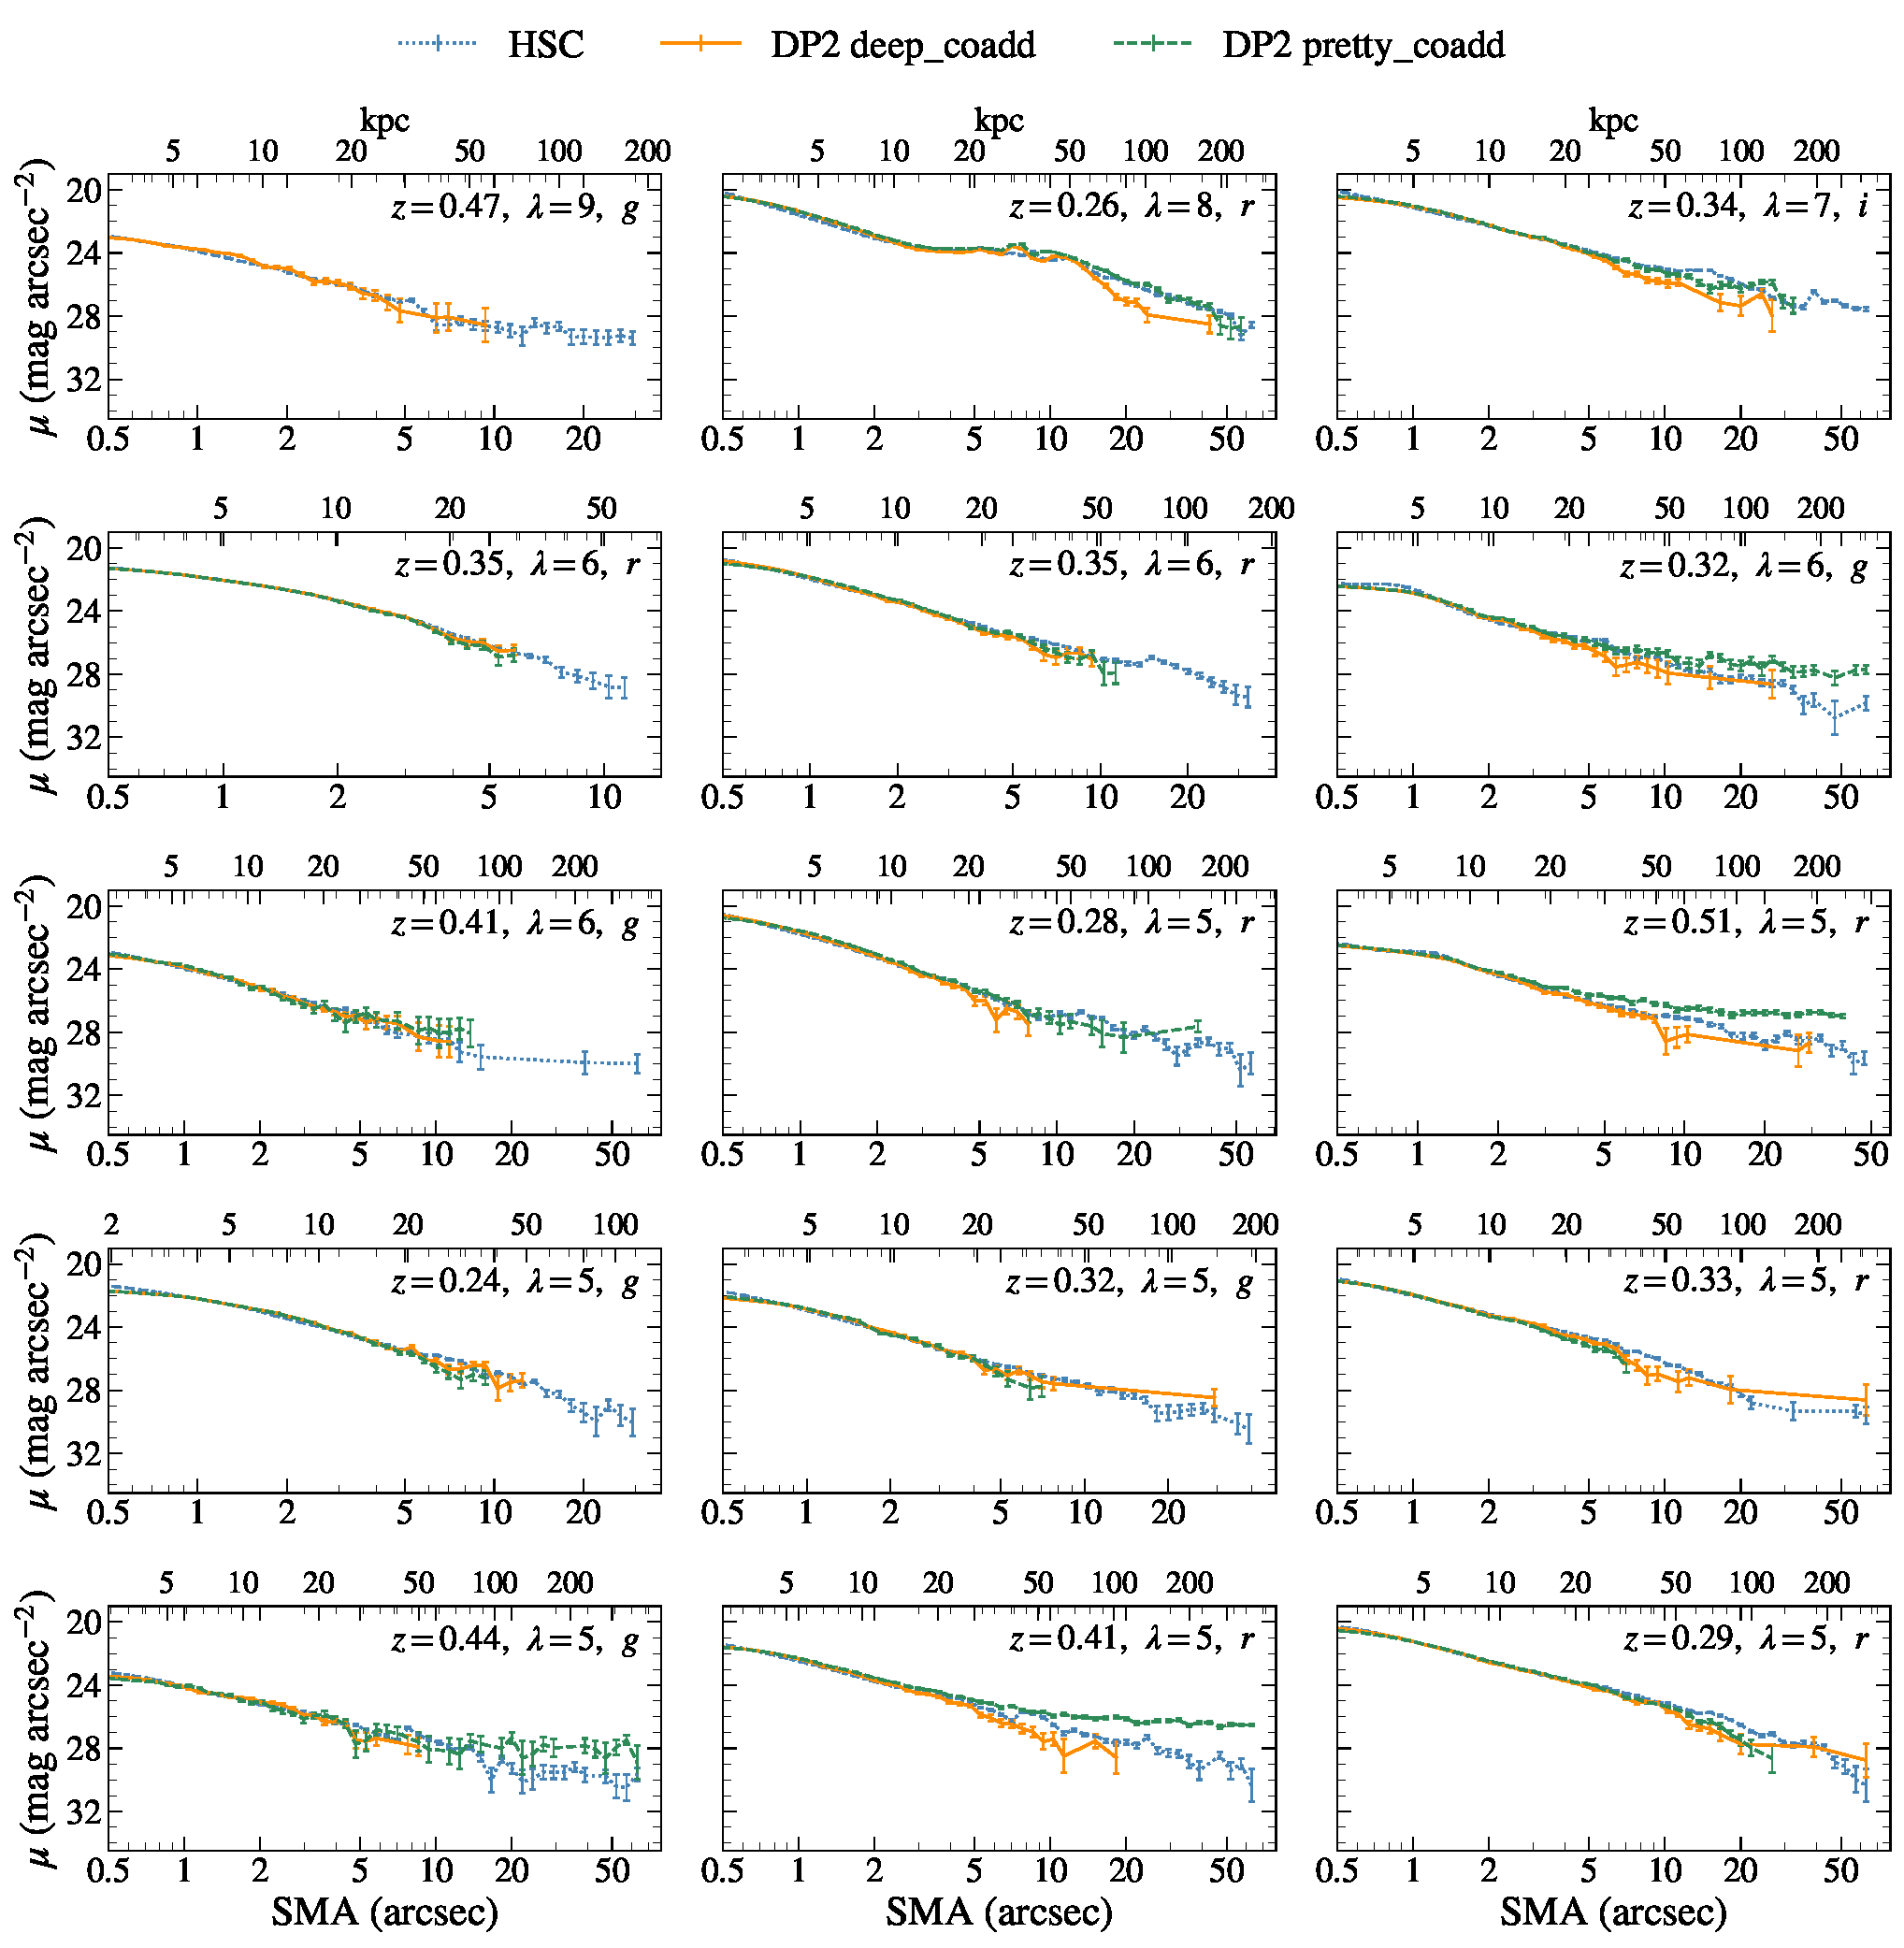
\includegraphics[width=1.0\linewidth]{figures/sbp_all.pdf}
  \caption{Surface brightness profiles of all 15 matched BCGs, ordered by decreasing richness. Each panel is labeled with the redshift, the richness, and the band in which the two surveys are compared. The panels share the surface brightness axis while the radial range is set per galaxy on a logarithmic axis. The top axis gives the projected physical scale in kpc for a Planck 2018 cosmology. Points carry $1\sigma$ uncertainties and only points with an intensity signal-to-noise ratio greater than 1 are shown. The \texttt{deep\_coadd} profiles end earlier than the HSC ones because background over-subtraction drives their outer intensity to zero. Several \texttt{pretty\_coadd} profiles instead stop declining and flatten into a plateau at large radii, well above the HSC profile of the same galaxy.}
  \label{fig:all}
\end{figure}

\section{Conclusion}
In this technote we performed elliptical isophote photometry on 15 massive BCGs in DP2 \texttt{deep\_coadd} and \texttt{pretty\_coadd} imaging. We used the same per-galaxy source masks and the same radial bins as the HSC photometry so that the two surveys are compared on a common pixel set. The \texttt{deep\_coadd} profiles match HSC at the center but are over-subtracted. They become progressively fainter than HSC outward by a median of $0.21$\,mag\,arcsec$^{-2}$ over $3''$--$40''$ and $0.5$\,mag\,arcsec$^{-2}$ beyond $10''$. Their intensity falls to zero at a median of $18''$, against $63''$ for HSC. The \texttt{pretty\_coadd} profiles reach further out but are not yet trustworthy there. In four of the eight galaxies where they extend beyond $20''$ they flatten into a plateau up to $2.1$\,mag\,arcsec$^{-2}$ brighter than HSC. We show this plateau to be the residual sky of the \texttt{pretty\_coadd}, an arcminute-scale ramp of a few nJy per pixel that the focal-plane sky correction leaves behind. The \texttt{deep\_coadd}'s coadd-level background removes that ramp together with the galaxy outskirts. Mosaicking adjacent patches to reach the outermost HSC bins for BCGs near patch boundaries does not change any \texttt{deep\_coadd} profile and only lengthens \texttt{pretty\_coadd} profiles that are dominated by residual sky, so it is not pursued here.

\appendix

\section{Acknowledgements}

This material is based upon work supported in part by the National Science Foundation through Cooperative Agreements AST-1258333 and AST-2241526 and Cooperative Support Agreements AST-1202910 and AST-2211468 managed by the Association of Universities for Research in Astronomy (AURA), and the Department of Energy under Contract No.\ DE-AC02-76SF00515 with the SLAC National Accelerator Laboratory managed by Stanford University.
Additional Rubin Observatory funding comes from private donations, grants to universities, and in-kind support from LSST-DA Institutional Members.

% Include all the relevant bib files.
% https://lsst-texmf.lsst.io/lsstdoc.html#bibliographies
\section{References} \label{sec:bib}
\renewcommand{\refname}{} % Suppress default Bibliography section
\bibliography{local,lsst,lsst-dm,refs_ads,refs,books}

% Make sure lsst-texmf/bin/generateAcronyms.py is in your path
\section{Acronyms} \label{sec:acronyms}
\input{acronyms.tex}
% If you want glossary uncomment below -- comment out the two lines above
%\printglossaries


\end{document}
